\documentclass[12pt]{article}

\usepackage{hyperref}
\usepackage{graphicx}
\usepackage{booktabs}
\usepackage{geometry}
\usepackage{tabularx}
\usepackage{float}
\usepackage[none]{hyphenat}
\usepackage{setspace}
\usepackage{subcaption}
\usepackage{titlesec}
\usepackage{amsmath}

\geometry{margin=1in}
\setstretch{0.96}

\titlespacing*{\section}{0pt}{10pt}{4pt}

\setlength{\parindent}{0pt}
\setlength{\parskip}{6pt}

\title{Labwork 1}
\author{Trinh Thanh Vinh - 2540110}
\date{\today}

\begin{document}

\maketitle

\section{Introduction}
In this labwork, we implement the linear regression algorithm using gradient descent to find the best-fitting line for a given dataset. We will analyze the convergence of the algorithm and observe how different learning rates affect the results.
\section{Implementation and Experimentation}
The dataset used in this labwork consists of pairs of \( (x, y) \) values, where \( x \) is the input feature and \( y \) is the target result. The goal of linear regression is to find the parameters \( w_1 \) and \( w_0 \) such that the line defined by \( y = w_1 x + w_0 \) best fits the data points. It also means that we want to find the \((w1, w0)\) that minimizes the loss function defined as the formula \( J = \frac{1}{n} \cdot \frac{1}{2} \sum_{i=1}^{n} (y_i - (w_1 x_i + w_0))^2 \), where \( n \) is the number of data points.

\begin{itemize}
    \item The loss function \( J(w_1, w_0) \) which we want to minimize.

    \item The derivative of the loss function with respect to \( w_1 \) and \( w_0 \), which are computed using the formulas:
    \[
    \frac{\partial J}{\partial w_1} = -\frac{1}{n} \sum_{i=1}^{n} x_i (y_i - (w_1 x_i + w_0))
    \]
    \[
    \frac{\partial J}{\partial w_0} = -\frac{1}{n} \sum_{i=1}^{n} (y_i - (w_1 x_i + w_0))
    \]

    \item The gradient descent algorithm that updates the values of \( w_1 \) and \( w_0 \) in each iteration, based on the computed gradient and a specified learning rate. The update stops when the change in the loss function is less than a specified threshold showing that the algorithm has converged to a minimum value.
\end{itemize}

\section{Results and Discussion}
With this problem, we set the initial values of \( w_1 \) and \( w_0 \) to 1 and 0 respectively. The initial learning rate is set to the same value as in the first labwork, which is 0.1. However, the algorithm does not converge as the \(w0\) and \(w1\) values diverge to infinity. Because of that, the learning rate is reduced to a much more smaller value at 0.0001, and the algorithm successfully converges to the optimal values of \( w_1 \) and \( w_0 \) after nearly 180000 steps, with \(w1\) being approximately 1.3, and \(w0\) being approximately 48. The resulting line is plotted against the original data points, showing a good fit to the data.
\begin{figure}[h]
    \centering
    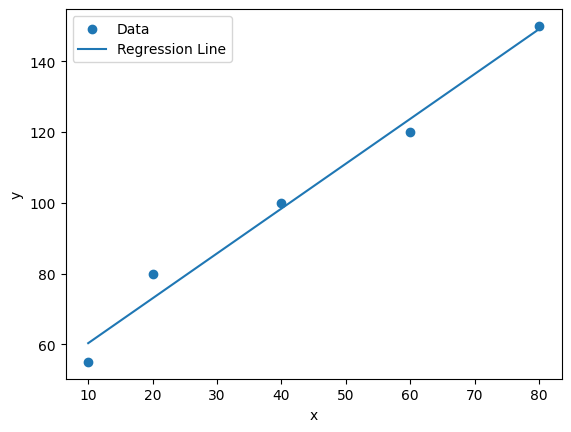
\includegraphics[width=0.8\textwidth]{figure.png}
    \caption{Data points and the fitted regression line}
\end{figure}

Similar to the first labwork, smaller learning rate is also used, which is 0.00005, and the algorithm successfully converges to the optimal values of \( w_1 \) and \( w_0 \) after over 333000 steps, with the same values of \( w_1 \) and \( w_0 \) as the previous case.

\end{document}